\appendix
\chapter{Appendinx: Meetin protocols} \label{sec:appendix}

\section{Meeting 01 - 15.10.2012}
The first meeting started with a presentation of the work of the \emph{Frauenhofer Institute}, which is part of the \emph{Frauenhofer Society}. The Frauenhofer Society is a German research organization with $60$ institutes spread throughout Germany, each focusing on different fields of applied science (as opposed to the Max Planck Society, which works primarily on basic science).

The course is guided by Prof. Dr. Ina Schieferdecker. Our project group works with three computer scientists from the Frauenhofer Fokus institute in Berlin (Tom Ritter, Christian Hein and Michael Wagner).

At this meeting, we first got a general introduction to model driven engineering. Therefore we reviewed learning methods of abstraction to focus on creating and exploiting domain models (that is, abstract representations of the knowledge and activities that govern a particular application domain), rather than on the computing (or algorithmic) concepts. We also got a small overview over the main software development processes (waterfall model, v-model and so on). Our first task for the following week should be to create an UML diagram with Papyrus for a generic firm.

\section{Meeting 02 - 22.10.20120}
We presented all solutions for the task with the firm. There where surprisingly different solutions for the task. So there were actually no right or wrong solutions. For example: An employee was a full-time, half-time or even external worker. We modeled that with having an enumeration containing those items. Others used inheritance to model such a system. The next task was to create an UML profile for this firm.

\section{Meeting 03 - 29.10.2012}
The solutions of the UML profile were not as expected. All teams had different profiles and although there is no right and wrong again everybody had problems with Papyrus. In many cases Eclipse just did not react to changes in the diagram or did not do the expected operations. Only one person had no problems with Eclipse, so this person presented its profile. So the difficulty was not to create the profile, but to get this plugin working.

\section{Meeting 04 - 05.11.2012}
The first meetings were like an introduction to model based engineering. We got a few tasks to do. In this meeting the project tasks were presented. There were a bunch of tasks. In most cases a tool for a special case was needed and so we should implement it. We wanted to take the Sonar task and we were lucky, because nobody else wanted to take this task. With the teams we made a small brainstorming to get a feeling for the task. In this brainstorming we collected our knowledge about static code analysis and especially Sonar. Because of the fact some team members already had worked with Sonar, they gave us a short introduction to code analysis with Sonar.

The task for the following week was to install and test Sonar and the Modelbus repository, which is a system containing models and source code, that should be analyzed with Sonar (that was our task). Another task was to work out some first requirements.

\section{Meeting 05 - 12.11.2012}
We presented the requirement list, which of course was not specific enough. We simply did not have much knowledge about the task and about plugin development for Sonar. Other teams had the same issue, their results were not specific as well.

The task for the following meeting was to specify the requirements more and to provide a first architecture concept. You can find the new requirement list here.

\section{Meeting 06 (Hackathon) - 23.11.2012}
The weekly meeting at university was not taking place this week, so we decided to meet and work together in the team. We therefore organized a hackathon, where we installed the software (some had build problems during the installation of the components). We also worked out an architecture concept and created a few diagrams to show our progress.

\section{Meeting 07 - 26.11.2012}
We presented our new requirements and the architecture. Our architecture concept was regarded to be good enough, so we are good to start the development of the plugin.

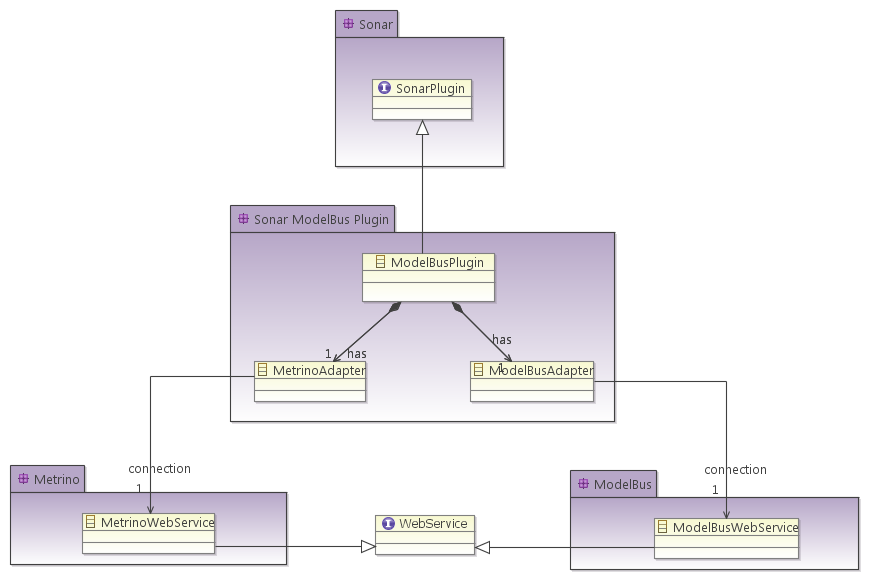
\includegraphics{architecture}